\documentclass[14pt, a4paper]{report}
\usepackage{mathtext}
\usepackage[T2A]{fontenc}
\usepackage[utf8]{inputenc}
\usepackage[russian]{babel}
\usepackage{multirow}
\usepackage{slashbox}
\usepackage{makecell}
\usepackage{graphicx}
\usepackage{physics}
\usepackage{amstext}
\usepackage{caption}
\usepackage{subcaption}
\usepackage{cmap}
\usepackage{float}
\usepackage{indentfirst}
\usepackage{romannum}
\usepackage{caption}

\usepackage[a4paper,
            		left=1in,
            		right=1in,
           		 top=1in,
            		bottom=1in,
            		footskip=.25in]{geometry}

\renewcommand{\thesection}{\arabic{section}.}
\renewcommand{\thesubsection}{\arabic{section}.\arabic{subsection}.}

\title{\textbf{Отчет о выполнении лабораторной работы 5.4.1 "Определение энергии $\alpha$-частиц по величине их пробега в воздухе"}}
\author{Калашников Михаил, Б03-202}
\date{}

\begin{document}
\maketitle

\pagenumbering{arabic}

\section{Экспериментальная установка}

\subsection{Счетчик Гейгера}

Для определения пробега $\alpha$-частиц с помощью счетчика, радиоактивный источник помещается на дно стальной цилиндрической бомбы, в которой может перемещаться торцевой счетчик Гейгера. Его чувствительный объем отделен от наружной среды тонким слюдяным окошком, сквозь которое могут проходить $\alpha$-частицы.

Импульсы, возникающие в счетчике, усиливаются и регистрируются пересчетной схемой. Путь частиц в воздухе зависит от расстояния между источником и счетчиком. Перемещение счетчика производится путем вращения гайки, находящейся на крышке бомбы. Расстояние между счетчиком и препаратом измеряется по шкале, нанесенной на держатель.

\subsection{Cцинтилляционный счетчик}

Установка состоит из цилиндрической камеры, на дне которой находится исследуемый препарат. Камера герметично закрыта
стеклянной пластинкой, на которую с внутренней стороны нанесен слой люминофора. С на ужной стороны к стеклу прижат
фотокатод фотоумножителя. Сигналы с фотоумножителя через усилитель поступают на пересчетную установку. Расстояние между
препаратом и люминофором составляет 9 см, так что $\alpha$-частицы не могут достигнуть люминофора при обычном давлении.
Определение пробега сводится к измерению зависимости интенсивности счета от давления в камере.

\subsection{Ионизационная камера}

Ионизационная камера -- прибор для количественного измерения ионизации, произведенной заряженными частицами при прохождении через газ. Камера представляет собой наполненный газом сосуд с дву-
мя электродами. Сферическая стенка прибора служит одним из электродов, второй электрод вводится в газ через изолирующую пробку. К электродам подводится постоянное напряжение от источника ЭДС. 

Заполняющий сосуд газ сам по себе не проводит электрический ток, возникает он только при прохождении быстрой заряженной частицы, которая рождает в газе на своем пути ионы.

\captionsetup{width=.25\textwidth}
\begin{figure}[H]
\centering
\begin{minipage}{.3\textwidth}
  \centering
  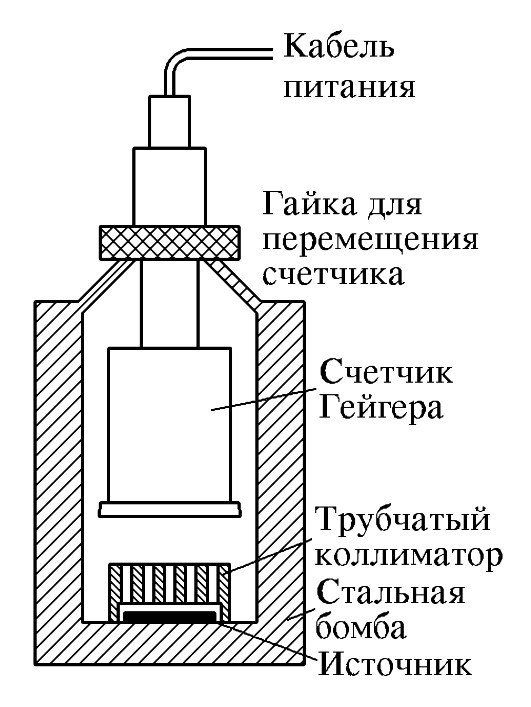
\includegraphics[width=.7\linewidth]{../images/541-1}
  \caption{Установка для измерения пробега $\alpha$-частиц с помощью торцевого счетчика Гейгера}
\end{minipage}%
\begin{minipage}{.3\textwidth}
  \centering
  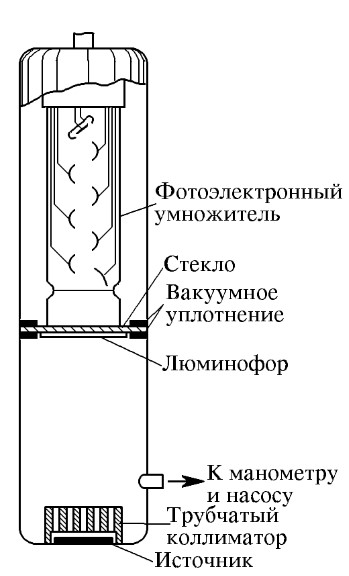
\includegraphics[width=.7\linewidth]{../images/541-2}
  \caption{Установка для измерения пробега $\alpha$-частиц с помощью стинцилляционного счетчика}
\end{minipage}%
\begin{minipage}{.3\textwidth}
  \centering
  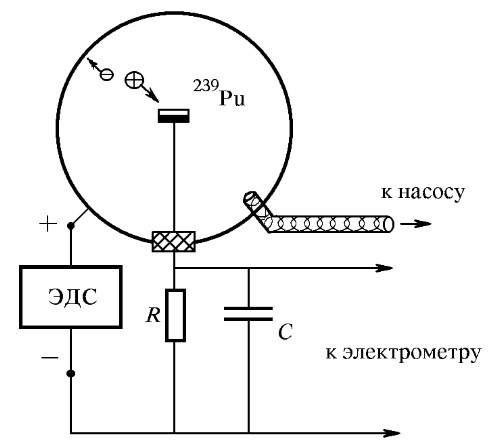
\includegraphics[width=.9\linewidth]{../images/541-3}
  \caption{Схема устройства ионизационной камеры}
\end{minipage}
\end{figure}
\captionsetup{width=.75\textwidth}

\newpage

\section{Проведение эксперимента и обработка результатов}

\subsection{Исследование пробега $\alpha$-частиц с помощью счетчика Гейгера}

Проведем измерения зависимости скорости счета от расстояния между источником и счетчиком, перемещая счетчик. Построим график $N(x)$. По графику определим значениe $R_{э}$. Сильный разброс экспериментальных точек не позволяет определить точку перегибра графика. Оценим $R_{ср}$ как среднюю точку линейной части зависимости.
 
\begin{figure}[H]
\centering
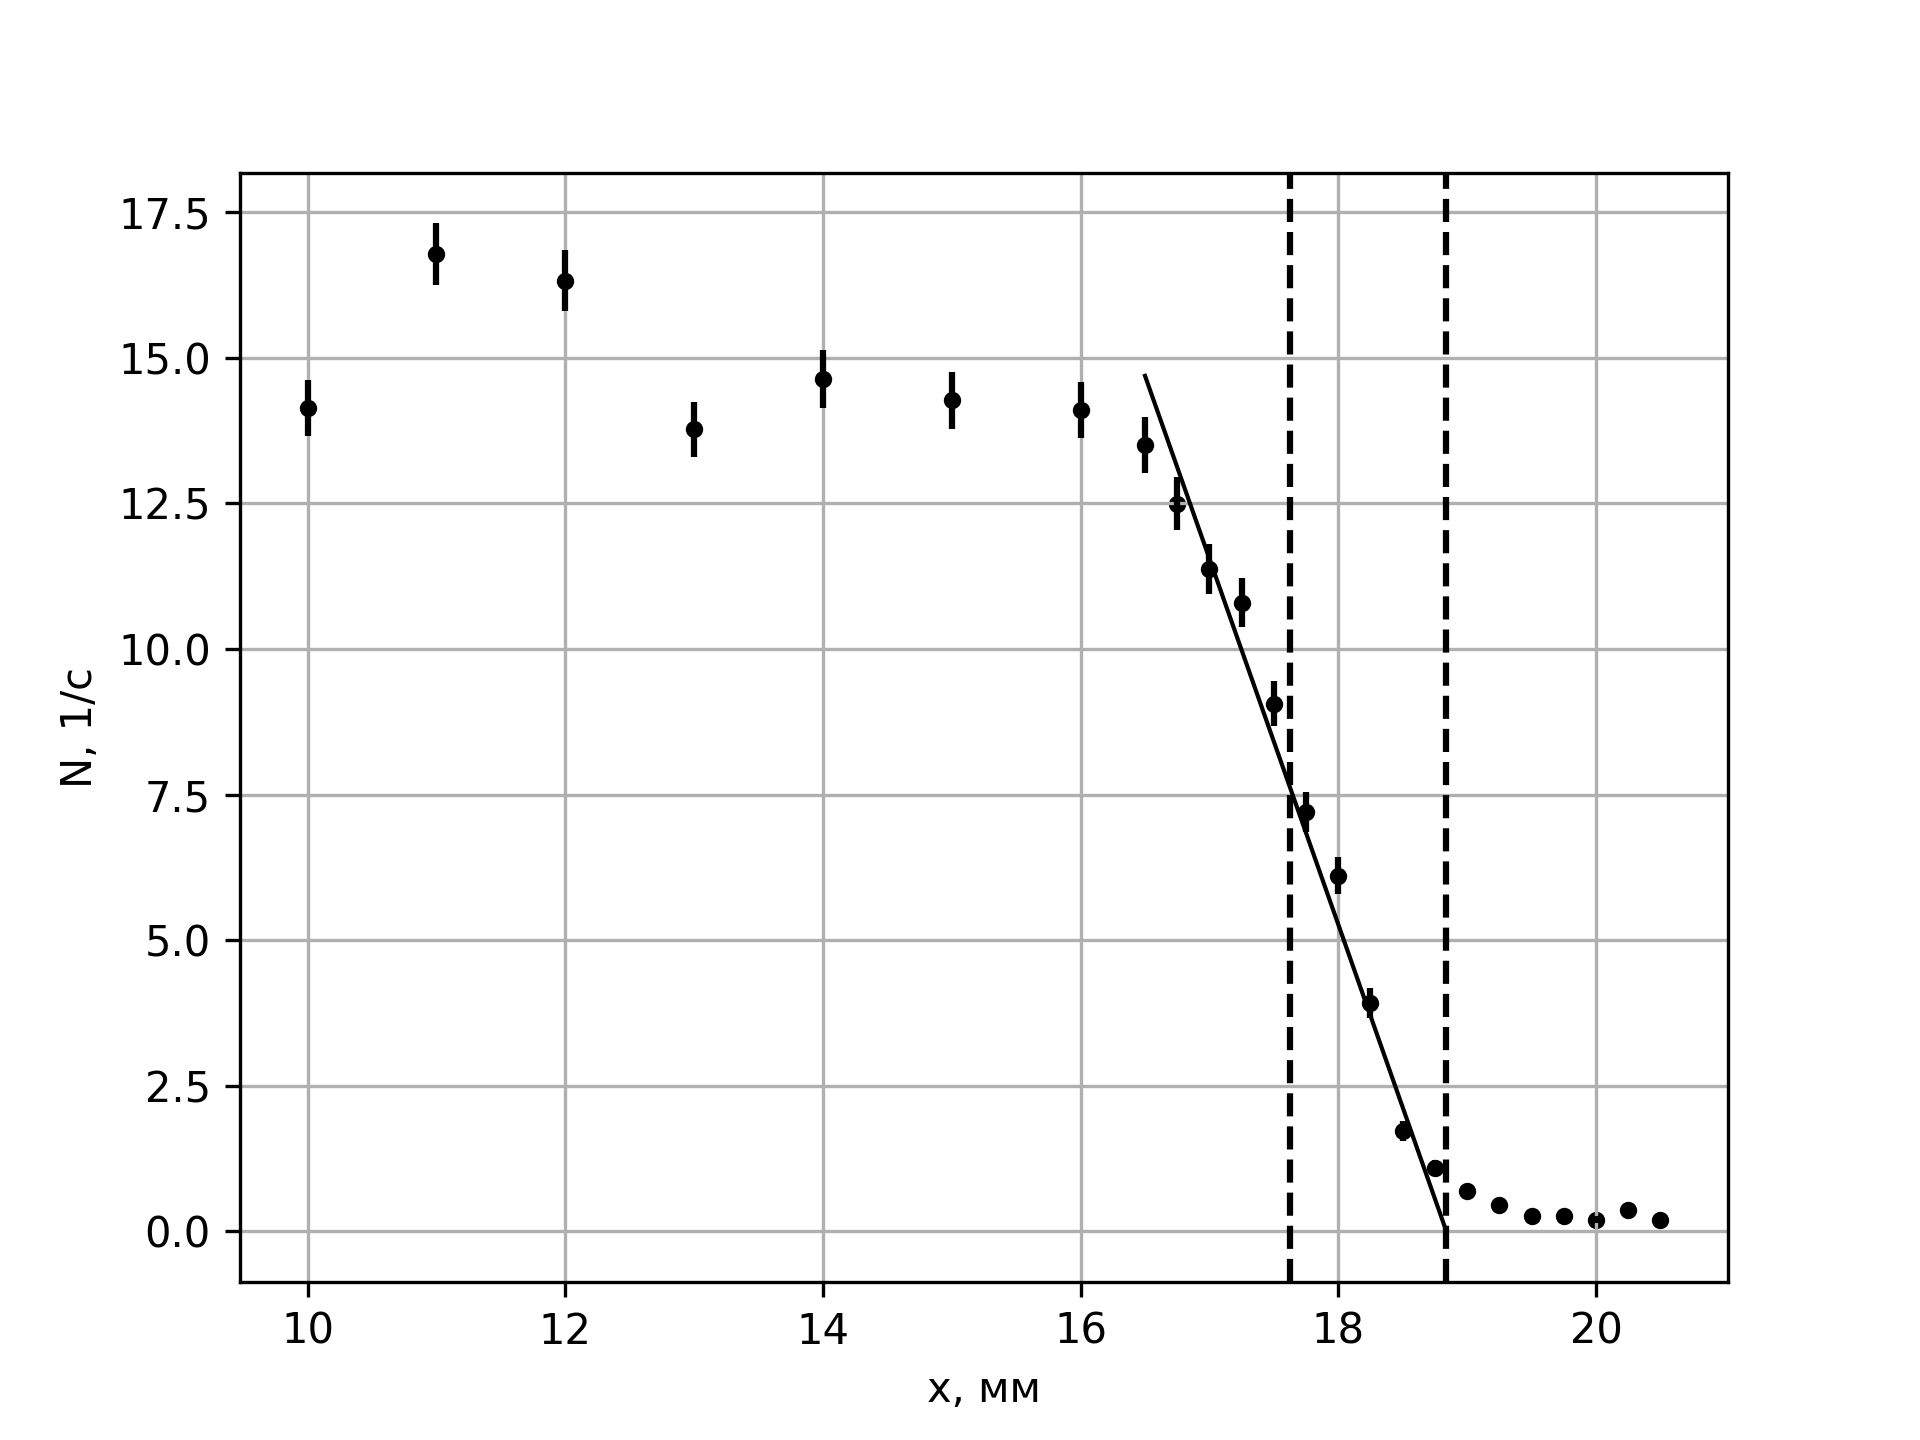
\includegraphics[width=.8\linewidth]{../images/541-4}
\caption{График зависимости $N(x)$ для счетчика Гейгера}
\end{figure}

\[R_{э}=(18.84\pm0.06)\ мм^{-1},\quad R_{ср}=(17.63\pm0.18)\ мм^{-1}\]
\[R'_{э}=(2.206\pm0.007)\ мг/см^2,\quad R'_{ср}=(2.06\pm0.02)\ мг/см^2\]

\newpage

\subsection{Определение пробега $\alpha$-частиц с помощью сцинтилляционного счетчика}

Проведем измерения зависимости скорости счета от давления в камере, перемещая счетчик. Построим график $N(P)$. По графику определим значениe $P_{э}$. Для определения $P_{ср}$ численно продифференцируем полученную зависимость. Пик производной аппроксимируем параболой и найдем положение ее вершины. Оно будет соответствовать $P_{ср}$. Зная, что расстояние между детектором и источником $x_0$ составляет 9 см, вычислим длину свободного пробега по формуле:

\[R=x_0\frac{P}{P_{норм}}\frac{T_{норм}}{T}\]

\begin{figure}[H]
\centering
\begin{minipage}{.8\textwidth}
  \centering
  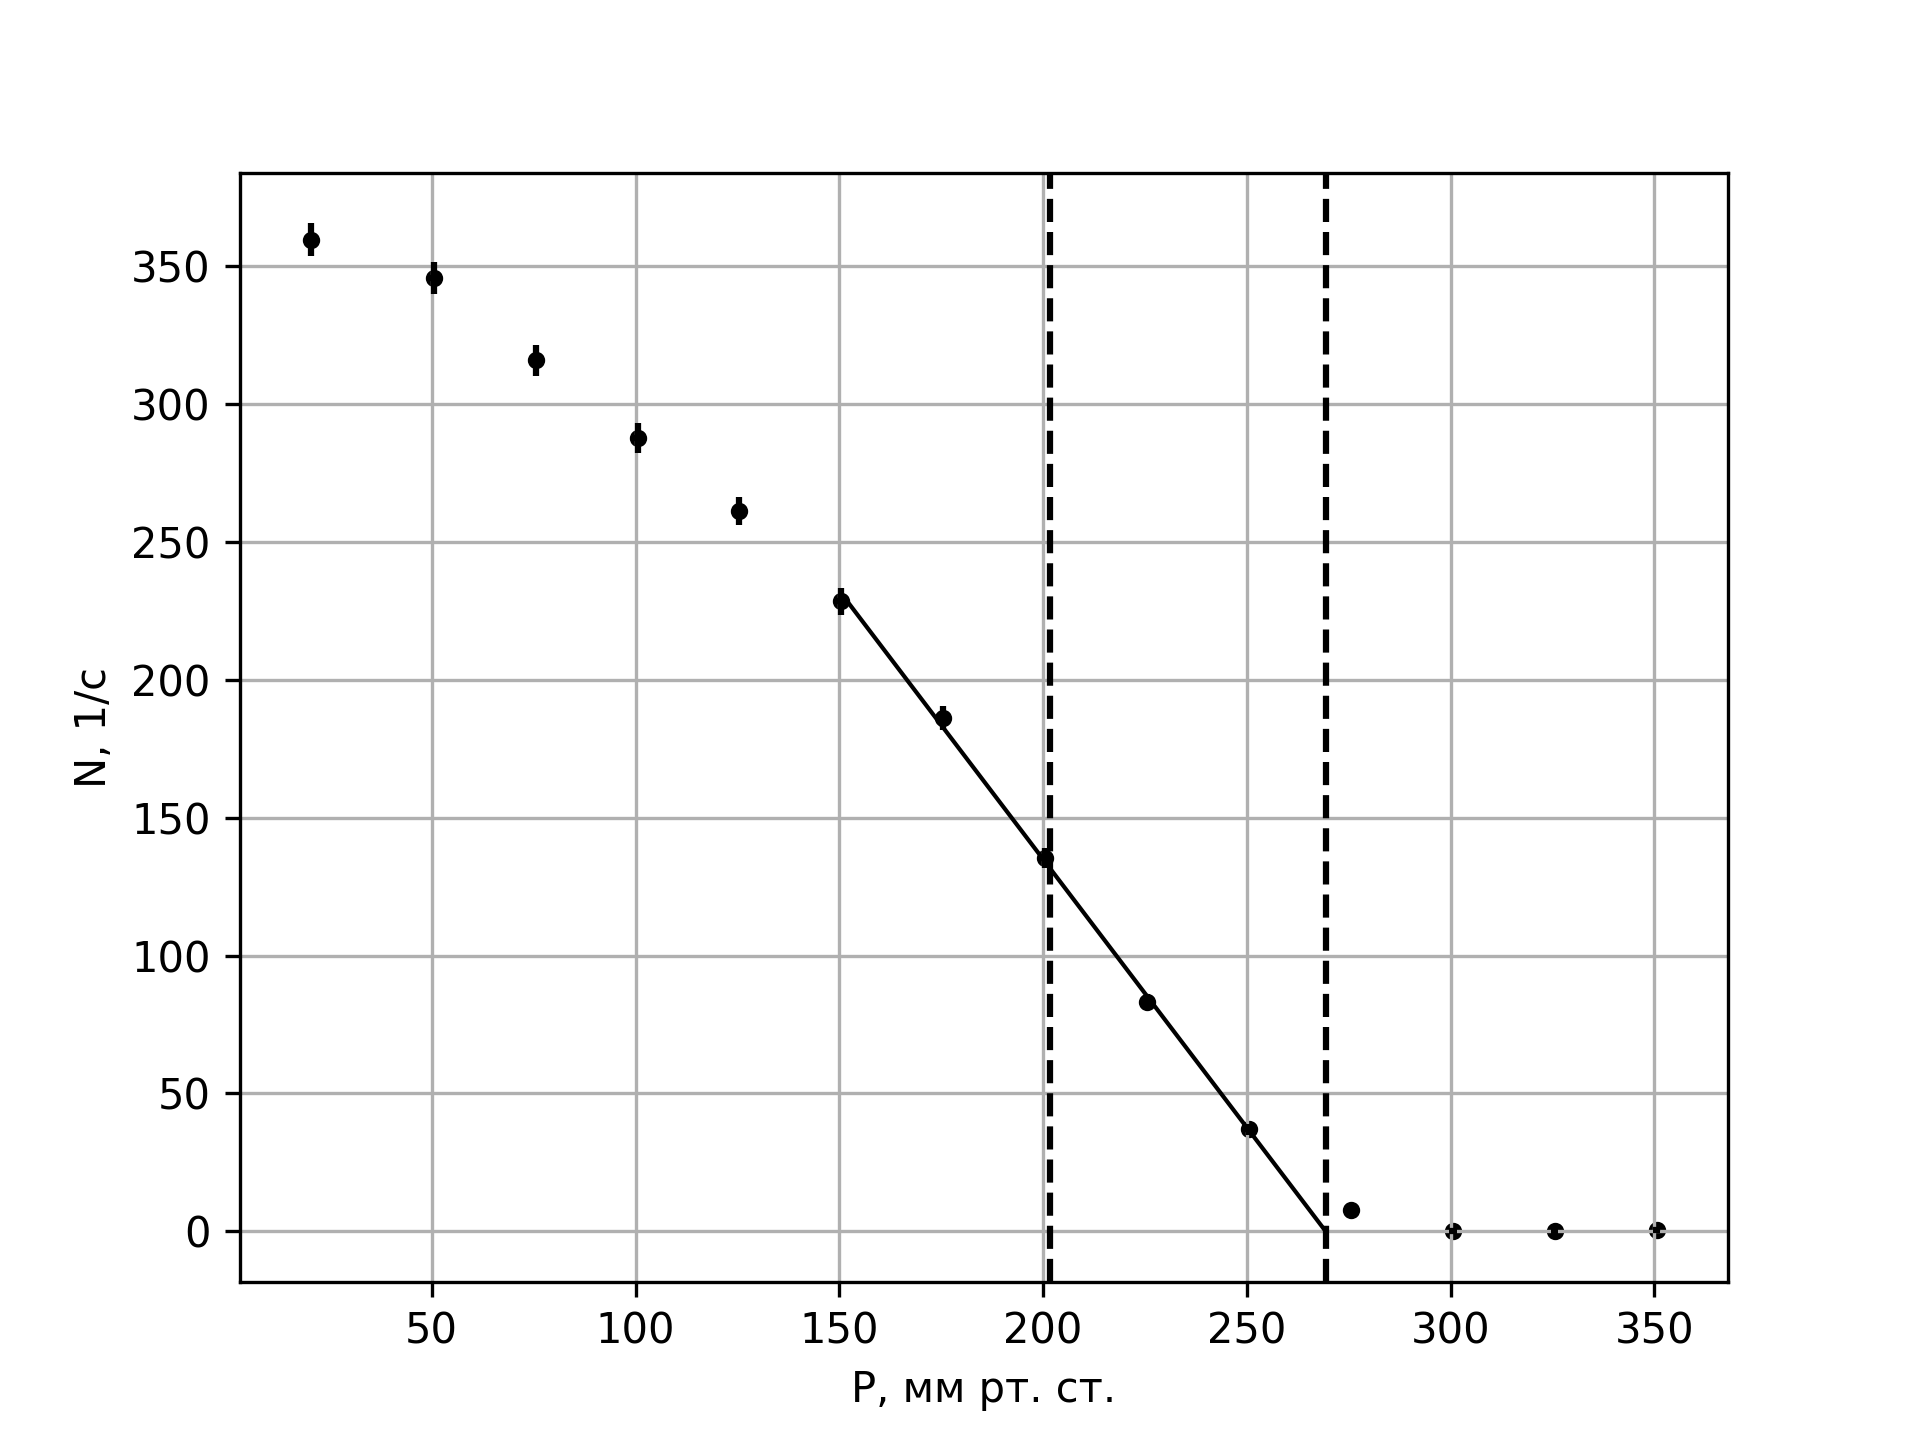
\includegraphics[width=.8\linewidth]{../images/541-5}
  \caption{График зависимости $N(P)$ для сцинтилляционной камеры}
\end{minipage}
\begin{minipage}{.8\textwidth}
  \centering
  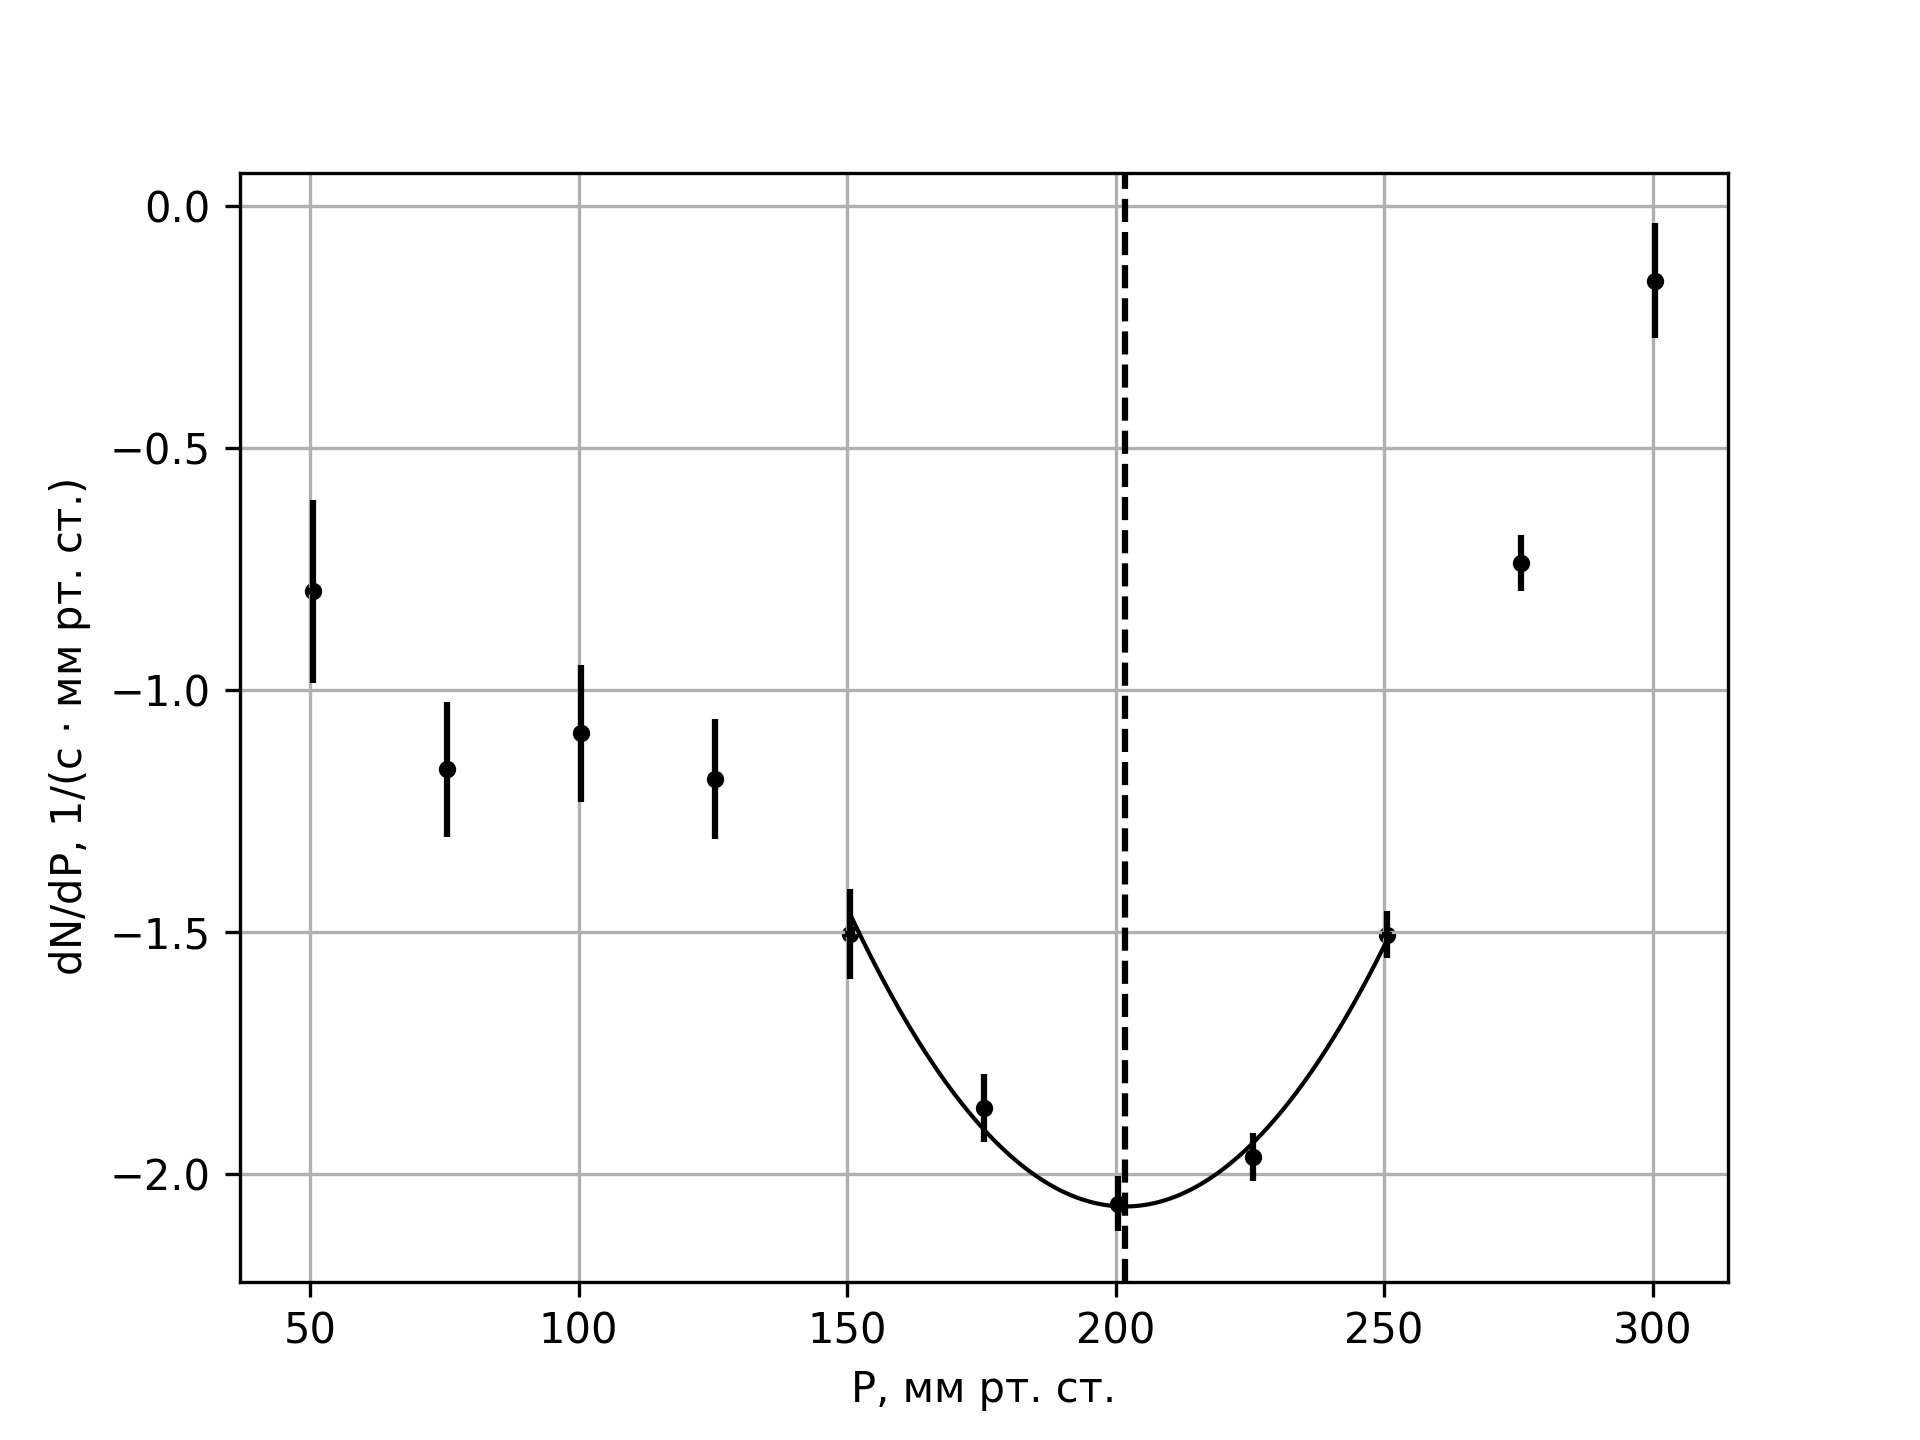
\includegraphics[width=.8\linewidth]{../images/541-6}
  \caption{График зависимости производной $N(P)$ для сцинтилляционной камеры}
\end{minipage}
\end{figure}

\[R_{э}=(30.82\pm0.10)\ мм^{-1},\quad R_{ср}=(23.09\pm0.15)\ мм^{-1}\]
\[R'_{э}=(1.295\pm0.004)\ мг/см^2,\quad R'_{ср}=(0.727\pm0.005)\ мг/см^2\]

\newpage

Определим толщину слюды, закрывающей окно торцевого счетчика.

\end{document}